\title{8 Goniometrické rovnice}
\author{Roman Šnajder}
\date{May 2025}


\maketitle

\section{Goniometrické rovnice}
\subsection{Základní goniometrické rovnice}
Rovnice v nichž se vyskytují goniometrické výrazy s neznámou $x\in R$ nazýváme goniometrické rovnice. Vzhledem k tomu, že jsou goniometrické funkce periodické, mohou mít goniometrické rovnice nekonečně mnoho kořenů. Stačí za k v $k\pi$ dosadit jakékoliv celé číslo.
$$\sin(x)=\frac{1}{2}$$
$$x=\frac{\pi}{6}$$
$$x_1=\frac{\pi}{6}+2k\pi$$
$$x_1=\frac{5\pi}{6}+2k\pi$$
Rovnice, ve kterých funkce nabývají hodnot mimo interval $\langle -1; 1 \rangle$ nemají řešení, jelikož se tato čísla nenacházejí na jednotkové kružnici. Například $\sin(x)=3$.
Tato rovnice $3\sin(x)=2$ však řešení má, jelikož jde obě strany vydělit číslem $3$ a dostaneme $\sin(x)=\frac{2}{3}$.
\subsection{Použití substituce u goniometrických rovnic}
$$2\sin(x)^2+\sin(x)-1=0$$ $$\sin(x)=t$$
$$2t^2+t-1=0$$
$$(t+1)\cdot(2t-1)=0$$
$$t_1=-1; t_2=\frac{1}{2}$$
$$\sin(x)=-1;\sin(x)=\frac{1}{2}$$
$$x_1=\frac{3}{2}+2k\pi$$
$$x_2=\frac{\pi}{6}+2k\pi;x_3=\frac{5\pi}{6}+2k\pi$$
Substituci lze využít i takto:
$$\sin(2x-\frac{\pi}{3})=1$$
$$2x-\frac{\pi}{3}=t$$
$$\sin(t)=1$$
$$t=\frac{\pi}{2}+2k\pi$$ 
$$2x-\frac{\pi}{3}=\frac{\pi}{2}+2k\pi$$
$$2x=\frac{5\pi}{6}+2k\pi$$
$$x=\frac{5\pi}{12}+k\pi$$
Goniometrické rovnice je možné řešit i za pomoci následujících vzorečků (zde jsou vypsány pouze některé vzorce):
$$\sin^2x+\cos^2x=1$$
$$tgx=\frac{\sin(x)}{\cos(x)}$$
$$cotgx=\frac{\cos(x)}{\sin(x)}$$
$$tgx-cotgx=1$$
$$\sin2x=2\cdot \sin(x)\cdot \cos(x)$$
$$\cos(2x)=\cos^2x-\sin^2x$$
\subsection{Kvadranty}
Každou goniometrickou funkci, která je definována v $\langle0; 2\pi\rangle$ lze znázornit na jednotkové kružnici, kde mezi každými dvěma osami je právě jeden kvadrant. V celku je tedy kružnice tvořena čtyřmi kvadranty a pomocí jedné hodnoty $(\frac{\pi}{6})$ v obloukové míře je možné dopočítat hodnoty ve zbylých kvadrantech $(\frac{5\pi}{6}); (\frac{7\pi}{6}); (\frac{11\pi}{6})$ opět v obloukových mírách.
Zde jsou pravidla pro výpočet daných hodnot $$x_1=x_0$$ $$x_2=\pi-x_0$$ $$x_2=\pi+x_0$$ $$x_2=2\pi-x_0$$
\subsubsection{Jednotková kružnice}
Vzdálenost od středu se vypočítá jako tangens úhlu nebo poměr protilehlé strany (sin osy y) ku přilehlé straně (cos osy x). V pravoúhlém trojúhelníku může tangens úhlu dosahovat libovolných kladných hodnot. Pohyb na grafu od $(0;\infty)$ se na jednotkové kružnici znázorní pohybem PROTI SMĚRU hodinových ručiček.
\begin{itemize}
    \item Funkce sinus v prvních dvou kvadrantech je kladná, v druhých dvou je záporná
    \item Funkce cosinus v prvním a čtvrtém kvadrantu roste, v druhém a třetím klesá 
    \item Funkce tangens je v první kvadrantu kladná a v druhém záporná
    \item Funkce kotangens je v prvním kvadrantu kladná a v druhém záporná
\end{itemize}
(1. kvadrant vpravo nahoře $(0;90^\circ)$; 2. kvadrant vlevo nahoře $(90^\circ;180^\circ)$; 3. kvadrant vlevo dole $(180^\circ;270^\circ)$; 4. kvadrant vpravo dole $(270^\circ;360^\circ)$)

\begin{figure}
    \centering
    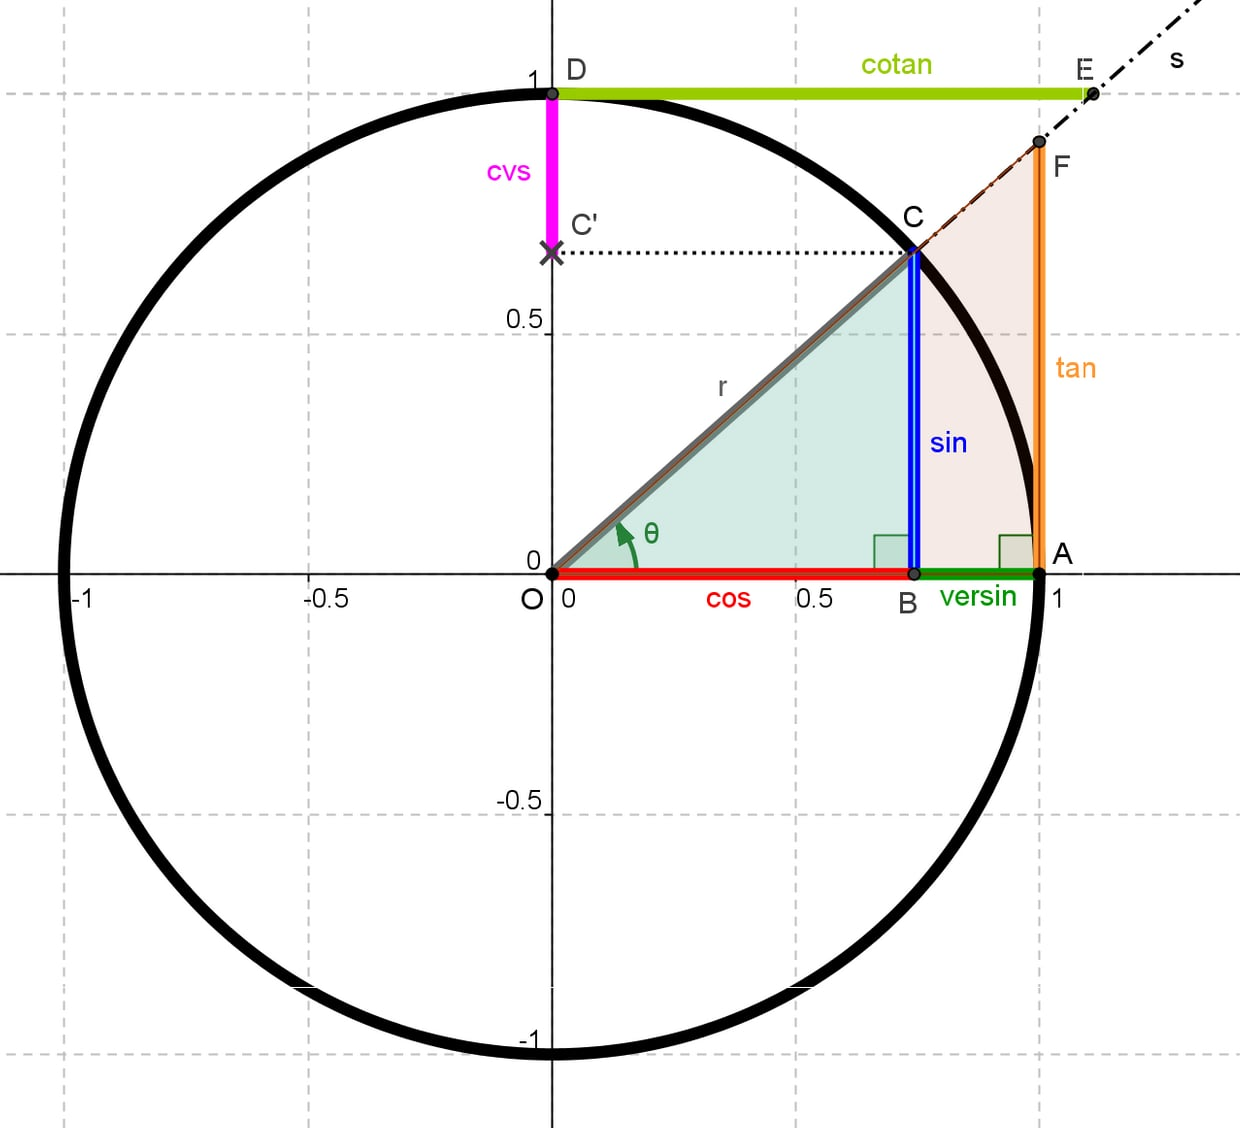
\includegraphics[width=0.5\linewidth]{img/jednotkova_Kruznice.jpg}
    \caption{Jednotková kružnice}
    \label{fig:enter-label}
\end{figure}


\begin{figure}
    \centering
    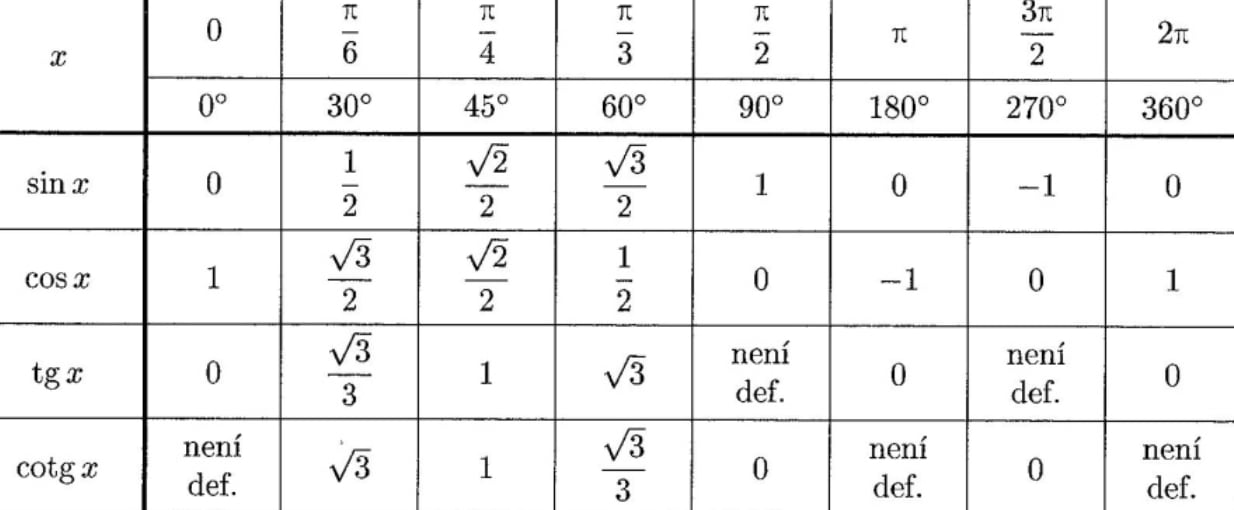
\includegraphics[width=1\linewidth]{img/tabulka_hodnot_goniometrickych.jpg}
    \caption{Tabulka hodnot goniometrických funkcí}
    \label{fig:enter-label}
\end{figure}

\subsection{Řešení rovnice ve stupních a převod mezi radiány a stupni}
Goniometrické rovnice mohu být řešeny buď v radiánech nebo ve stupních – záleží na zadání. Zde jsou vzorečky pro převody mezi stupni a radiány.

\begin{itemize}
    \item Ze stupňů na radiány: $\alpha$ rad=$\frac{\pi}{180\textdegree}\cdot\alpha$ stupně
\\ například $30^\circ$ na radiány
$$
    30^\circ \cdot\frac{\pi}{180^\circ}=\frac{\pi}{6}
$$
    \item Z radiánů na stupně: $\alpha$ stupně=$\frac{180\textdegree}{\pi}\cdot\alpha$ rad
\\ například $\frac{\pi}{2}$ na stupně
$$
    \frac{\pi}{2} \cdot 180^\circ=90^\circ
$$
\end{itemize}

Rovnice zadaná ve stupních $\sin(x)=\frac{\pi}{2}$, $x\in\langle0 ^\circ;360^\circ \rangle$
$$\sin(x)=\frac{\pi}{2} \rightarrow x=30^\circ$$
$$x_1=30$$
$$x_2=180^\circ-30^\circ\Rightarrow150^\circ$$
\subsection{Řešení rovnice v daném intervalu}
Pokud je goniometrická rovnice zadána s konkrétním intervalem, musí být řešena právě v tomto intervalu. Po výpočtu všech možných řešení je nutné tato řešení porovnat s daným intervalem a zapsat pouze ta, která do něj skutečně náleží.
Rovnice $cosx=-\frac{\pi}{2}$, $x\in\langle\frac{\pi}{2};\frac{3\pi}{2}\rangle$
$$x_1=\pi-\frac{\pi}{3}\Rightarrow\frac{2\pi}{3}$$
$$x_2=\pi+\frac{\pi}{3}\Rightarrow\frac{4\pi}{3}$$
